% Created with jtex v.1.0.20
\documentclass{article}
\usepackage{hyperref}
\usepackage{datetime}
\usepackage{graphicx}
\usepackage{natbib}
\bibliographystyle{abbrvnat}

%%%%%%%%%%%%%%%%%%%%%%%%%%%%%%%%%%%%%%%%%%%%%%%%%%
%%%%%%%%%%%%%%%%%%%%  imports  %%%%%%%%%%%%%%%%%%%
\usepackage{booktabs}
%%%%%%%%%%%%%%%%%%%%%%%%%%%%%%%%%%%%%%%%%%%%%%%%%%


% colors for hyperlinks
\hypersetup{colorlinks=true, allcolors=blue}

\newcommand{\logo}{
  \href{https://curvenote.com}{
\includegraphics[width=2cm]{curvenote.png}}
}

\title{K-means Analysis}

\author{Sunghyun Ahn \and Megan Dhillon \and Yoohan Park \and Breitling Snyder}

\newdate{articleDate}{18}{12}{2025}
\date{\displaydate{articleDate}}

\begin{document}
\maketitle
\begin{center}\logo\end{center}


\begin{verbatim}
import pandas as pd
import geopandas as gpd
import matplotlib.pyplot as plt

import sys
sys.path.append("..")
from CEStools.utils import clean_data

import numpy as np
from sklearn.preprocessing import StandardScaler
from sklearn.cluster import KMeans
from sklearn.metrics import silhouette_score
\end{verbatim}

\begin{verbatim}
# Import and clean the data
df_raw = pd.read_csv('../data/calenviroscreen40.csv')

df_clean = clean_data(df_raw)
X = df_clean[df_clean.notna().all(axis=1)]
\end{verbatim}

\begin{itemize}
\item CalEnviroScreen uses \texttt{-999} and \texttt{-1998} as \textit{sentinel values} meaning ``missing'' or ``not applicable''.
\item We create a boolean mask that keeps only rows where \textbf{all} entries do not include \texttt{-999} and \texttt{-1998}.
\item The cleaned DataFrame is stored in \texttt{X}.
\item We print the number of original vs. cleaned rows to see how many tracts were removed.
\end{itemize}

\begin{verbatim}
print(f"Original rows: {len(df_clean):,}")
print(f"Clean rows   : {len(X):,}")
\end{verbatim}

\begin{verbatim}
Original rows: 8,035
Clean rows   : 7,354
\end{verbatim}

\begin{verbatim}
X
\end{verbatim}

\bigskip\noindent
\begin{tabular}{p{\dimexpr 0.045\linewidth-2\tabcolsep}p{\dimexpr 0.045\linewidth-2\tabcolsep}p{\dimexpr 0.045\linewidth-2\tabcolsep}p{\dimexpr 0.045\linewidth-2\tabcolsep}p{\dimexpr 0.045\linewidth-2\tabcolsep}p{\dimexpr 0.045\linewidth-2\tabcolsep}p{\dimexpr 0.045\linewidth-2\tabcolsep}p{\dimexpr 0.045\linewidth-2\tabcolsep}p{\dimexpr 0.045\linewidth-2\tabcolsep}p{\dimexpr 0.045\linewidth-2\tabcolsep}p{\dimexpr 0.045\linewidth-2\tabcolsep}p{\dimexpr 0.045\linewidth-2\tabcolsep}p{\dimexpr 0.045\linewidth-2\tabcolsep}p{\dimexpr 0.045\linewidth-2\tabcolsep}p{\dimexpr 0.045\linewidth-2\tabcolsep}p{\dimexpr 0.045\linewidth-2\tabcolsep}p{\dimexpr 0.045\linewidth-2\tabcolsep}p{\dimexpr 0.045\linewidth-2\tabcolsep}p{\dimexpr 0.045\linewidth-2\tabcolsep}p{\dimexpr 0.045\linewidth-2\tabcolsep}p{\dimexpr 0.045\linewidth-2\tabcolsep}p{\dimexpr 0.045\linewidth-2\tabcolsep}}
\toprule
 & CIscoreP & OzoneP & PM2\_5\_P & DieselPM\_P & PesticideP & Tox\_Rel\_P & TrafficP & DrinkWatP & Lead\_P & CleanupP & ... & PovertyP & UnemplP & HousBurdP & PopCharP & Hispanic & White & AfricanAm & NativeAm & OtherMult & AAPI \\
\hline
0 & 69.162885 & 10.566273 & 10.031114 & 52.408214 & 92.034483 & 9.914979 & 63.4000 & 11.165230 & 36.118463 & 17.077268 & ... & 89.660804 & 18.310776 & 69.150824 & 79.828543 & 68.9210 & 20.8899 & 0.4004 & 0.2670 & 1.3126 & 8.2091 \\
\hline
1 & 70.637922 & 11.561917 & 10.454263 & 39.365277 & 99.586207 & 10.265066 & 19.9000 & 52.828775 & 43.805923 & 72.396417 & ... & 83.040201 & 69.130661 & 60.101394 & 56.555724 & 78.6229 & 13.2240 & 2.5051 & 0.0000 & 0.9489 & 4.6990 \\
\hline
2 & 61.069087 & 10.566273 & 9.931549 & 60.311139 & 93.827586 & 10.515129 & 42.7500 & 11.165230 & 75.072464 & 2.071669 & ... & 52.876884 & 35.020822 & 53.624842 & 67.183560 & 65.7214 & 30.6088 & 0.9591 & 0.0000 & 2.1685 & 0.5421 \\
\hline
3 & 5.988401 & 13.615432 & 10.653391 & 34.275047 & 95.413793 & 7.864466 & 39.9250 & 32.559011 & 11.077505 & 0.000000 & ... & 7.550251 & 58.355023 & 16.311787 & 10.741301 & 22.9537 & 69.1948 & 0.9342 & 0.7117 & 2.5356 & 3.6699 \\
\hline
4 & 23.121533 & 13.615432 & 10.690728 & 18.481643 & 63.241379 & 7.714429 & 24.3625 & 32.559011 & 49.514808 & 2.071669 & ... & 35.150754 & 92.399792 & 12.002535 & 46.280888 & 33.4082 & 59.7804 & 0.6986 & 1.4721 & 1.3723 & 3.2685 \\
\hline
... & ... & ... & ... & ... & ... & ... & ... & ... & ... & ... & ... & ... & ... & ... & ... & ... & ... & ... & ... & ... & ... \\
\hline
8030 & 30.610187 & 88.699440 & 72.109521 & 12.433105 & 0.000000 & 69.217304 & 18.7625 & 66.866492 & 80.340265 & 19.914147 & ... & 31.733668 & 1.900052 & 40.899873 & 22.339889 & 28.7132 & 53.3995 & 1.5733 & 0.0000 & 7.1549 & 9.1590 \\
\hline
8031 & 22.566818 & 79.987554 & 70.242688 & 21.306783 & 0.000000 & 70.430108 & 57.9875 & 73.148495 & 52.715816 & 5.636432 & ... & 41.030151 & 30.882353 & 52.610900 & 16.502774 & 10.9507 & 26.3918 & 3.3677 & 0.0000 & 3.3677 & 55.9221 \\
\hline
8032 & 74.508321 & 84.579963 & 72.906036 & 90.914748 & 0.000000 & 74.356089 & 79.2625 & 60.334707 & 57.996219 & 94.438223 & ... & 57.298995 & 59.383134 & 29.721166 & 43.582955 & 58.2273 & 16.1438 & 8.9967 & 0.0000 & 1.1098 & 15.5223 \\
\hline
8033 & 97.049924 & 46.994400 & 79.452396 & 42.265090 & 0.000000 & 91.047762 & 62.4000 & 71.362558 & 94.820416 & 74.300112 & ... & 91.557789 & 82.326913 & 64.461343 & 92.939990 & 91.4114 & 6.9425 & 0.6728 & 0.2577 & 0.7157 & 0.0000 \\
\hline
8034 & 97.226425 & 50.541381 & 79.775980 & 97.510890 & 67.586207 & 90.897724 & 98.0750 & 61.833396 & 97.391304 & 82.232176 & ... & 88.316583 & 83.224883 & 70.532319 & 76.727181 & 91.0941 & 1.3147 & 1.9084 & 0.0000 & 0.0000 & 5.6828 \\
\hline
\bottomrule
\end{tabular}

\bigskip

7354 rows $\times$ 30 columns

\begin{itemize}
\item K-means is distance-based, so features with larger scales can dominate the distance computation.
\item We use \texttt{StandardScaler} to transform each feature to have:

\begin{itemize}
\item mean $\approx$ 0
\item standard deviation $\approx$ 1
\end{itemize}


\item The scaled feature matrix is stored in \texttt{X\_scaled}.
\item For each \texttt{k} from 2 to 10:

\begin{itemize}
\item Fit a \texttt{KMeans} model on \texttt{X\_scaled} with:

\begin{itemize}
\item \texttt{random\_state=42} for reproducibility
\item \texttt{n\_init=10} to run the algorithm multiple times and keep the best solution.
\end{itemize}


\item Store the \textbf{inertia} (within-cluster sum of squared distances) in \texttt{inertias}.
\item Compute the \textbf{silhouette score} (how well-separated the clusters are) and store it in \texttt{sil\_scores}.
\end{itemize}
\end{itemize}

\begin{verbatim}
# Standardize the features
scaler = StandardScaler()
X_scaled = scaler.fit_transform(X.values)
\end{verbatim}

\begin{verbatim}
# Run KMeans for k = 2,...,10 and compute inertia + silhouette score
k_values = list(range(2, 11))
inertias = []
sil_scores = []

for k in k_values:
    kmeans = KMeans(
        n_clusters=k,
        random_state=42,  # set random state for reproducibility
        n_init=10
    )
    labels = kmeans.fit_predict(X_scaled)
    inertias.append(kmeans.inertia_)
    sil_scores.append(silhouette_score(X_scaled, labels))
\end{verbatim}

\begin{verbatim}
# Plot: Elbow (Inertia) + Silhouette on twin axes
fig, ax1 = plt.subplots()

# Inertia line (left y -axis)
ax1.plot(
    k_values, inertias,
    marker="o",
    color="tab:blue",
    label="Inertia"
)
ax1.set_xlabel("Number of Clusters k")
ax1.set_ylabel("Inertia", color="tab:blue")
ax1.tick_params(axis="y", labelcolor="tab:blue")
ax1.set_title("Elbow Method vs. Silhouette Score")
ax1.grid(alpha=0.3, linestyle=" - -")  # light grid

# Silhouette line (right y -axis)
ax2 = ax1.twinx()
ax2.plot(
    k_values, sil_scores,
    marker="s",
    linestyle=" - -",
    color="tab:green",
    label="Silhouette Score"
)
ax2.set_ylabel("Silhouette Score", color="tab:green")
ax2.tick_params(axis="y", labelcolor="tab:green")

# Combine legends from both axes
lines1, labels1 = ax1.get_legend_handles_labels()
lines2, labels2 = ax2.get_legend_handles_labels()
ax1.legend(lines1 + lines2, labels1 + labels2, loc="best")

plt.tight_layout()
plt.savefig("../visualizations/kmeans_visualizations/elbowvssilohuette_chart.png", dpi=300, bbox_inches="tight")

plt.show()
\end{verbatim}

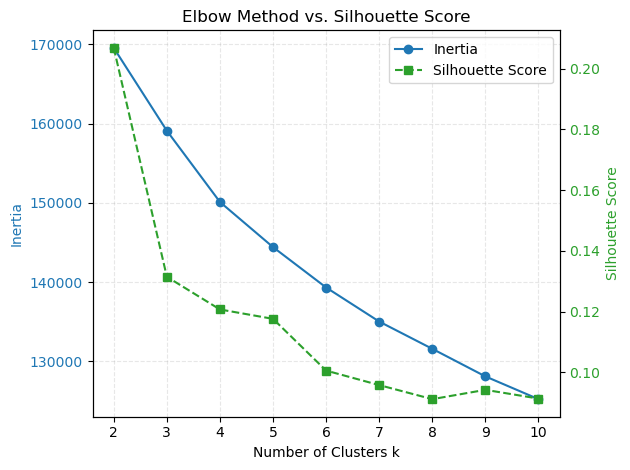
\includegraphics[width=0.7\linewidth]{files/6081317cf6029984a4e1bb90a86cbdaf.png}

\section{Interpretation: Elbow \& Silhouette Plot}

\begin{itemize}
\item The \textbf{inertia curve} (blue) decreases as we increase \texttt{k}, with diminishing returns after a certain point.
\item The \textbf{silhouette curve} (green) shows how well-separated the clusters are for each \texttt{k}.
\item We choose the value of \texttt{k} with the highest silhouette score (here, \texttt{k = 2}), balancing model fit and cluster separation.
\end{itemize}

\begin{verbatim}
feature_cols = ['CIscoreP', 'OzoneP',  'PM2_5_P', 'DieselPM_P', 'PesticideP',
                 'Tox_Rel_P', 'TrafficP', 'DrinkWatP', 'Lead_P', 'CleanupP',
                 'GWThreatP', 'HazWasteP', 'ImpWatBodP', 'SolWasteP', 'PolBurdP',
                 'AsthmaP', 'LowBirWP', 'CardiovasP', 'EducatP', 'Ling_IsolP',
                 'PovertyP', 'UnemplP', 'HousBurdP', 'PopCharP', 
                'Hispanic', 'White', 'AfricanAm', 'NativeAm', 'OtherMult', 'AAPI']

# Fit final model with best k (=2) based on silhouette
best_k = k_values[sil_scores.index(max(sil_scores))]
print(f"\nBest k based on silhouette score: {best_k}")

final_kmeans_2 = KMeans(
    n_clusters=best_k,
    random_state=42,
    n_init=10
)
final_labels_2 = final_kmeans_2.fit_predict(X_scaled)

cluster_centers = pd.DataFrame(
    final_kmeans_2.cluster_centers_,
    columns=feature_cols
)

cluster_centers
\end{verbatim}

\begin{verbatim}
Best k based on silhouette score: 2
\end{verbatim}

\bigskip\noindent
\begin{tabular}{p{\dimexpr 0.045\linewidth-2\tabcolsep}p{\dimexpr 0.045\linewidth-2\tabcolsep}p{\dimexpr 0.045\linewidth-2\tabcolsep}p{\dimexpr 0.045\linewidth-2\tabcolsep}p{\dimexpr 0.045\linewidth-2\tabcolsep}p{\dimexpr 0.045\linewidth-2\tabcolsep}p{\dimexpr 0.045\linewidth-2\tabcolsep}p{\dimexpr 0.045\linewidth-2\tabcolsep}p{\dimexpr 0.045\linewidth-2\tabcolsep}p{\dimexpr 0.045\linewidth-2\tabcolsep}p{\dimexpr 0.045\linewidth-2\tabcolsep}p{\dimexpr 0.045\linewidth-2\tabcolsep}p{\dimexpr 0.045\linewidth-2\tabcolsep}p{\dimexpr 0.045\linewidth-2\tabcolsep}p{\dimexpr 0.045\linewidth-2\tabcolsep}p{\dimexpr 0.045\linewidth-2\tabcolsep}p{\dimexpr 0.045\linewidth-2\tabcolsep}p{\dimexpr 0.045\linewidth-2\tabcolsep}p{\dimexpr 0.045\linewidth-2\tabcolsep}p{\dimexpr 0.045\linewidth-2\tabcolsep}p{\dimexpr 0.045\linewidth-2\tabcolsep}p{\dimexpr 0.045\linewidth-2\tabcolsep}}
\toprule
 & CIscoreP & OzoneP & PM2\_5\_P & DieselPM\_P & PesticideP & Tox\_Rel\_P & TrafficP & DrinkWatP & Lead\_P & CleanupP & ... & PovertyP & UnemplP & HousBurdP & PopCharP & Hispanic & White & AfricanAm & NativeAm & OtherMult & AAPI \\
\hline
0 & 0.886505 & 0.231807 & 0.502308 & 0.355547 & -0.033506 & 0.389607 & 0.123718 & 0.351488 & 0.656137 & 0.258066 & ... & 0.763402 & 0.454328 & 0.603947 & 0.852096 & 0.786568 & -0.760642 & 0.272985 & -0.064769 & -0.438613 & -0.164873 \\
\hline
1 & -0.789853 & -0.206534 & -0.447543 & -0.316783 & 0.029853 & -0.347129 & -0.110230 & -0.313167 & -0.584601 & -0.229930 & ... & -0.680171 & -0.404795 & -0.538101 & -0.759195 & -0.700812 & 0.677713 & -0.243223 & 0.057707 & 0.390793 & 0.146898 \\
\hline
\bottomrule
\end{tabular}

\bigskip

2 rows $\times$ 30 columns

\section{Interpretation : Cluster centers for k=2 (standardized scale)}

\begin{itemize}
\item \textbf{Cluster 0}: shows positive standardized scores across CalEnviroScreen percentiles for pollution burden (e.g., PM2.5, Diesel PM, Pollution Burden), health outcomes (AsthmaP, CardiovasP), and socioeconomic vulnerability (PovertyP, UnemplP, PopCharP), while having a strongly negative deviation for White population share. This cluster can be interpreted as high-burden, high-vulnerability, minority-majority communities.
\item \textbf{Cluster 1}:  in contrast, exhibits negative standardized values for most environmental, health, and vulnerability indicators, and a positive deviation for White population share. This cluster corresponds to low-burden, more advantaged, White-majority communities.
\end{itemize}

\begin{itemize}
\item We select the value of \texttt{k} = 2  that gives the \textbf{maximum silhouette score}.
\item Using this \texttt{best\_k}, we fit a final \texttt{KMeans} model on \texttt{X\_scaled}:

\begin{itemize}
\item The final cluster assignments for each tract are stored in \texttt{final\_labels}.
\item The standardized cluster means (centers) are stored in \texttt{cluster\_centers} as a DataFrame.
\end{itemize}


\item Each entry in \texttt{cluster\_centers} is a \textbf{z-score}:

\begin{itemize}
\item Positive values (\textgreater  0) mean the cluster has above-average levels for that feature.
\item Negative values (\textless  0) mean below-average levels for that feature.
\end{itemize}
\end{itemize}

\begin{verbatim}
# 1) Convert cluster centers into a DataFrame
cluster_centers = pd.DataFrame(
    final_kmeans_2.cluster_centers_,
    columns=feature_cols
)

# 2) Sort features by how different they are across clusters
#    (sort by variance across cluster means, descending)
feature_order = cluster_centers.var(axis=0).sort_values(ascending=False).index
cluster_centers_ord = cluster_centers[feature_order]

# 3) Draw the heatmap

fig, ax = plt.subplots(figsize=(min(0.5 * len(feature_order) + 3, 18), 3 + best_k))

im = ax.imshow(cluster_centers_ord, aspect="auto")

# Set x and y tick labels

ax.set_xticks(range(len(feature_order)))
ax.set_xticklabels(feature_order, rotation=90)

ax.set_yticks(range(best_k))
ax.set_yticklabels([f"Cluster {i}" for i in range(best_k)])

ax.set_title("Cluster Profile Heatmap (Standardized Means)")
ax.set_xlabel("Features")
ax.set_ylabel("Clusters")

# Add colorbar
cbar = fig.colorbar(im, ax=ax)
cbar.set_label("Standardized mean (z -score)")

plt.tight_layout()
plt.savefig("../visualizations/kmeans_visualizations/cluster_heatmap_2.png", dpi=300, bbox_inches="tight")

plt.show()
\end{verbatim}

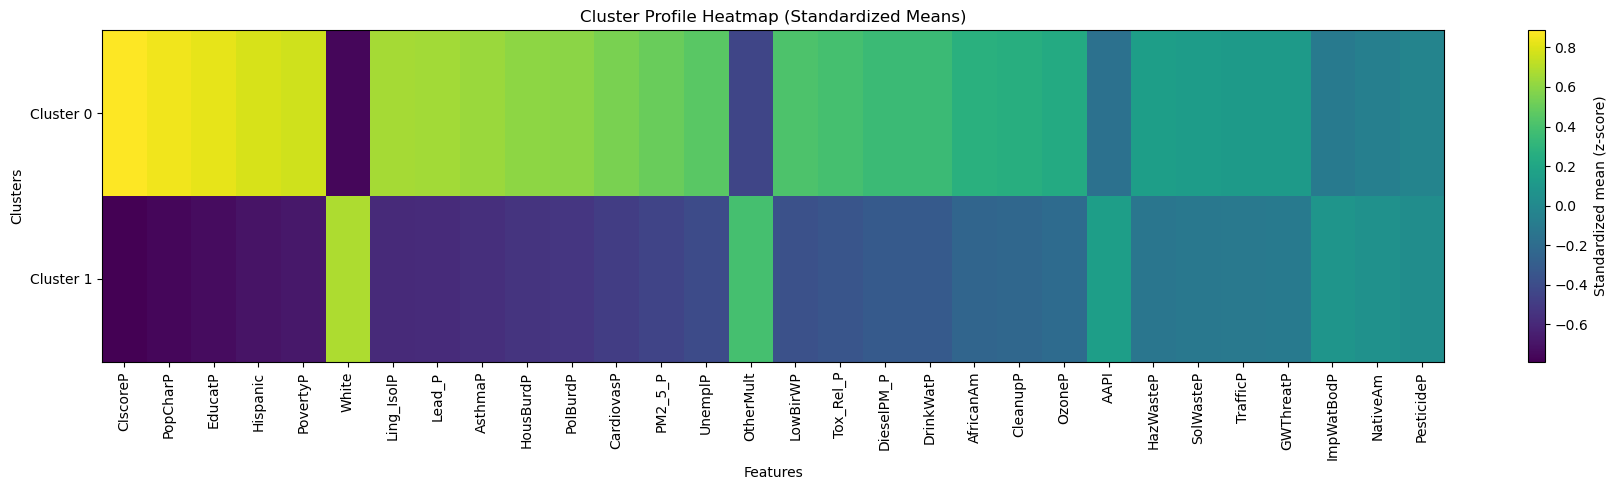
\includegraphics[width=0.7\linewidth]{files/b3589875fa67aeaf7b13a2977b5d114e.png}

\subsection{Cluster profile heatmap (k=2)}

The heatmap above shows the standardized cluster means (z-scores) for all CalEnviroScreen indicators and race-composition variables.

\begin{itemize}
\item Each row corresponds to one cluster (Cluster 0 and Cluster 1).
\item Each column is a feature (e.g., CIscoreP, PolBurdP, PovertyP, PM2\_5\_P, White, etc.).
\item Colors represent standardized means:

\begin{itemize}
\item Yellow / light colors indicate \textbf{above-average} values (positive z-scores).
\item Purple / dark colors indicate \textbf{below-average} values (negative z-scores).
\end{itemize}
\end{itemize}

We see a very clear pattern:

\begin{itemize}
\item \textbf{Cluster 0} has high values for \texttt{CIscoreP}, \texttt{PolBurdP}, \texttt{PM2\_5\_P}, \texttt{DieselPM\_P}, \texttt{AsthmaP}, \texttt{CardiovasP}, \texttt{PovertyP}, \texttt{UnemplP}, \texttt{PopCharP}, and other vulnerability metrics, while having a strongly negative value for White.\newline
\rightarrow This cluster represents \textbf{high-burden, high-vulnerability, minority-majority communities}.
\item \textbf{Cluster 1} shows the opposite pattern: most environmental and socioeconomic burden indicators are below average, while \texttt{White} is above average.\newline
\rightarrow This cluster represents \textbf{low-burden, more advantaged, White-majority communities}.
\end{itemize}

Features near zero in both clusters (e.g., GWThreatP, ImpWatBodP, PesticideP) do not strongly differentiate between clusters.

\begin{verbatim}
final_kmeans_4 = KMeans(
    n_clusters=4,
    random_state=42,
    n_init=10
)
final_labels_4 = final_kmeans_4.fit_predict(X_scaled)

cluster_centers = pd.DataFrame(
    final_kmeans_4.cluster_centers_,
    columns=feature_cols
)

cluster_centers
\end{verbatim}

\bigskip\noindent
\begin{tabular}{p{\dimexpr 0.045\linewidth-2\tabcolsep}p{\dimexpr 0.045\linewidth-2\tabcolsep}p{\dimexpr 0.045\linewidth-2\tabcolsep}p{\dimexpr 0.045\linewidth-2\tabcolsep}p{\dimexpr 0.045\linewidth-2\tabcolsep}p{\dimexpr 0.045\linewidth-2\tabcolsep}p{\dimexpr 0.045\linewidth-2\tabcolsep}p{\dimexpr 0.045\linewidth-2\tabcolsep}p{\dimexpr 0.045\linewidth-2\tabcolsep}p{\dimexpr 0.045\linewidth-2\tabcolsep}p{\dimexpr 0.045\linewidth-2\tabcolsep}p{\dimexpr 0.045\linewidth-2\tabcolsep}p{\dimexpr 0.045\linewidth-2\tabcolsep}p{\dimexpr 0.045\linewidth-2\tabcolsep}p{\dimexpr 0.045\linewidth-2\tabcolsep}p{\dimexpr 0.045\linewidth-2\tabcolsep}p{\dimexpr 0.045\linewidth-2\tabcolsep}p{\dimexpr 0.045\linewidth-2\tabcolsep}p{\dimexpr 0.045\linewidth-2\tabcolsep}p{\dimexpr 0.045\linewidth-2\tabcolsep}p{\dimexpr 0.045\linewidth-2\tabcolsep}p{\dimexpr 0.045\linewidth-2\tabcolsep}}
\toprule
 & CIscoreP & OzoneP & PM2\_5\_P & DieselPM\_P & PesticideP & Tox\_Rel\_P & TrafficP & DrinkWatP & Lead\_P & CleanupP & ... & PovertyP & UnemplP & HousBurdP & PopCharP & Hispanic & White & AfricanAm & NativeAm & OtherMult & AAPI \\
\hline
0 & 0.163023 & 0.315260 & -0.357524 & -0.491246 & 0.451294 & -0.599798 & -0.559154 & -0.033611 & -0.084915 & -0.327967 & ... & 0.485245 & 0.513885 & 0.043427 & 0.563190 & 0.243830 & -0.087735 & 0.168028 & 0.242361 & 0.036419 & -0.377593 \\
\hline
1 & -1.195938 & -0.229747 & -0.604225 & -0.678470 & 0.089290 & -0.529550 & -0.350217 & -0.439827 & -0.794830 & -0.447555 & ... & -0.949510 & -0.570933 & -0.793418 & -1.108066 & -0.849991 & 1.039094 & -0.384304 & 0.033895 & 0.377490 & -0.108950 \\
\hline
2 & 1.180867 & 0.304916 & 0.853813 & 0.572936 & -0.195983 & 0.725536 & 0.277460 & 0.593590 & 0.966809 & 0.450978 & ... & 0.957071 & 0.507591 & 0.836477 & 1.041357 & 1.113518 & -0.992137 & 0.287438 & -0.121336 & -0.703313 & -0.303633 \\
\hline
3 & -0.126892 & -0.369961 & 0.028404 & 0.564096 & -0.279100 & 0.307955 & 0.586114 & -0.149492 & -0.124495 & 0.290071 & ... & -0.442104 & -0.385137 & -0.088387 & -0.424706 & -0.525911 & 0.022339 & -0.036511 & -0.114567 & 0.348564 & 0.821319 \\
\hline
\bottomrule
\end{tabular}

\bigskip

4 rows $\times$ 30 columns

\begin{verbatim}
# 1) Convert cluster centers into a DataFrame
cluster_centers = pd.DataFrame(
    final_kmeans_4.cluster_centers_,
    columns=feature_cols
)

# 2) Sort features by how different they are across clusters
#    (sort by variance across cluster means, descending)
feature_order = cluster_centers.var(axis=0).sort_values(ascending=False).index
cluster_centers_ord = cluster_centers[feature_order]

# 3) Draw the heatmap

fig, ax = plt.subplots(figsize=(min(0.5 * len(feature_order) + 3, 18), 3 + 4))

im = ax.imshow(cluster_centers_ord, aspect="auto")

# Set x and y tick labels

ax.set_xticks(range(len(feature_order)))
ax.set_xticklabels(feature_order, rotation=90)

ax.set_yticks(range(4))
ax.set_yticklabels([f"Cluster {i}" for i in range(4)])

ax.set_title("Cluster Profile Heatmap (Standardized Means)")
ax.set_xlabel("Features")
ax.set_ylabel("Clusters")

# Add colorbar
cbar = fig.colorbar(im, ax=ax)
cbar.set_label("Standardized mean (z -score)")

plt.tight_layout()
plt.savefig("../visualizations/kmeans_visualizations/cluster_heatmap_4.png", dpi=300, bbox_inches="tight")

plt.show()
\end{verbatim}

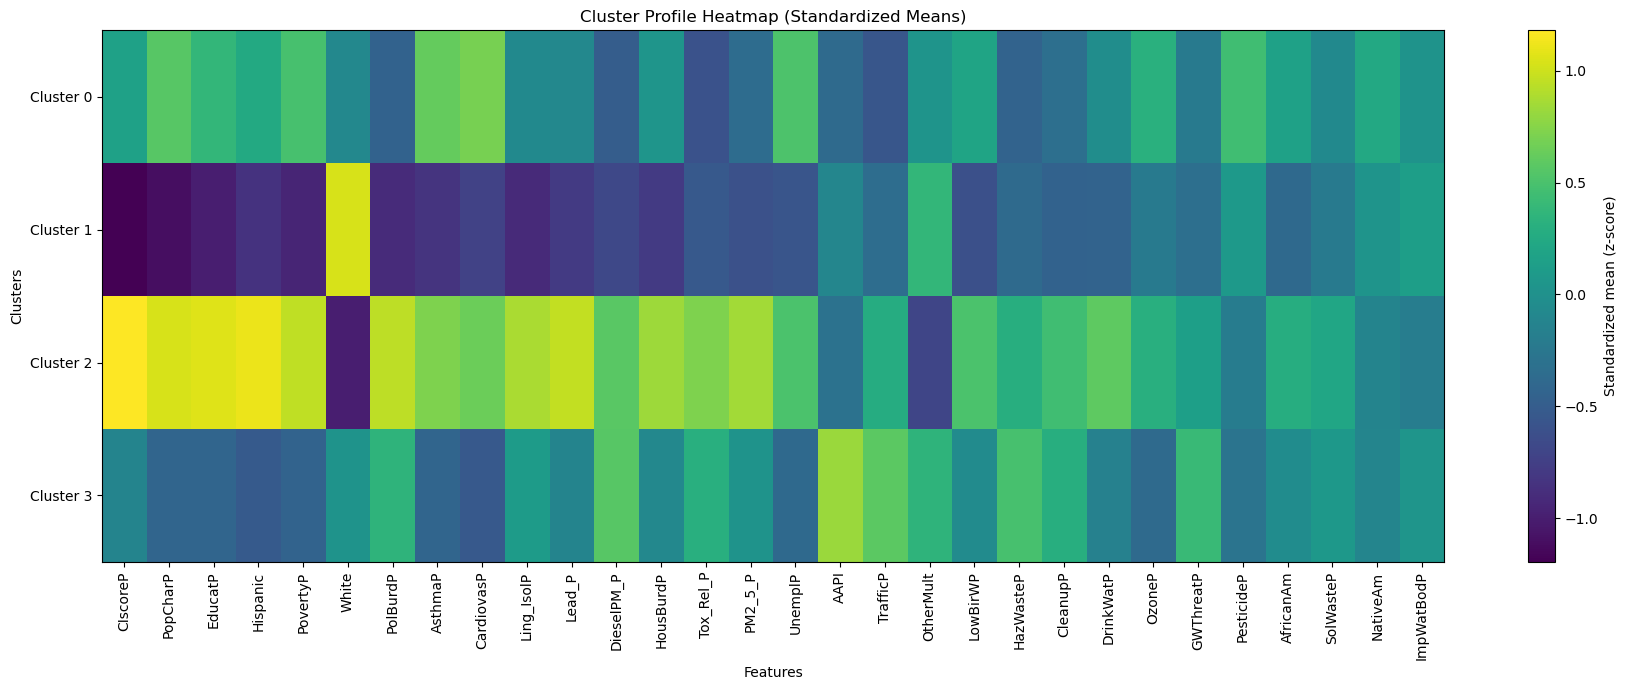
\includegraphics[width=0.7\linewidth]{files/37bfe3910e4a114d211fcf00261da0b9.png}

\subsection{Cluster profile heatmap (k=4)}

The heatmap above shows the standardized cluster means (z-scores) for all CalEnviroScreen indicators and race-composition variables.

\begin{itemize}
\item Each row corresponds to one cluster (Clusters 0,  1, 2, and 3).
\item Each column is a feature (e.g., CIscoreP, PolBurdP, PovertyP, PM2\_5\_P, White, etc.).
\item Colors represent standardized means:

\begin{itemize}
\item Yellow / light colors indicate \textbf{above-average} values (positive z-scores).
\item Purple / dark colors indicate \textbf{below-average} values (negative z-scores).
\end{itemize}
\end{itemize}

\begin{verbatim}
shp_path = "../data/calenviroscreen40_shp/CES4 Final Shapefile.shp"
shape = gpd.read_file(shp_path)

shape = clean_data(shape, keep_geom=True)
shape = shape[df_clean.notna().all(axis=1)]
shape = shape.to_crs(epsg=3857)
\end{verbatim}

\begin{verbatim}
cluster_labels_2 = pd.Series(final_labels_2, index=X.index, name="cluster_2")
cluster_labels_4 = pd.Series(final_labels_4, index=X.index, name="cluster_4")

clusters_df = pd.concat(
    [cluster_labels_2, cluster_labels_4],
    axis=1
)

gdf = shape.join(clusters_df)
\end{verbatim}

\begin{verbatim}
ax = gdf.plot(
    column="cluster_2",
    categorical=True,
    legend=True,
    figsize=(10, 12),
    linewidth=0.05,
    edgecolor="white"
)

ax.set_title("California Census Tracts by K -Means Cluster")
ax.set_axis_off()

plt.savefig("../visualizations/kmeans_visualizations/cluster_map_2.png", dpi=300, bbox_inches="tight")
plt.show()
\end{verbatim}

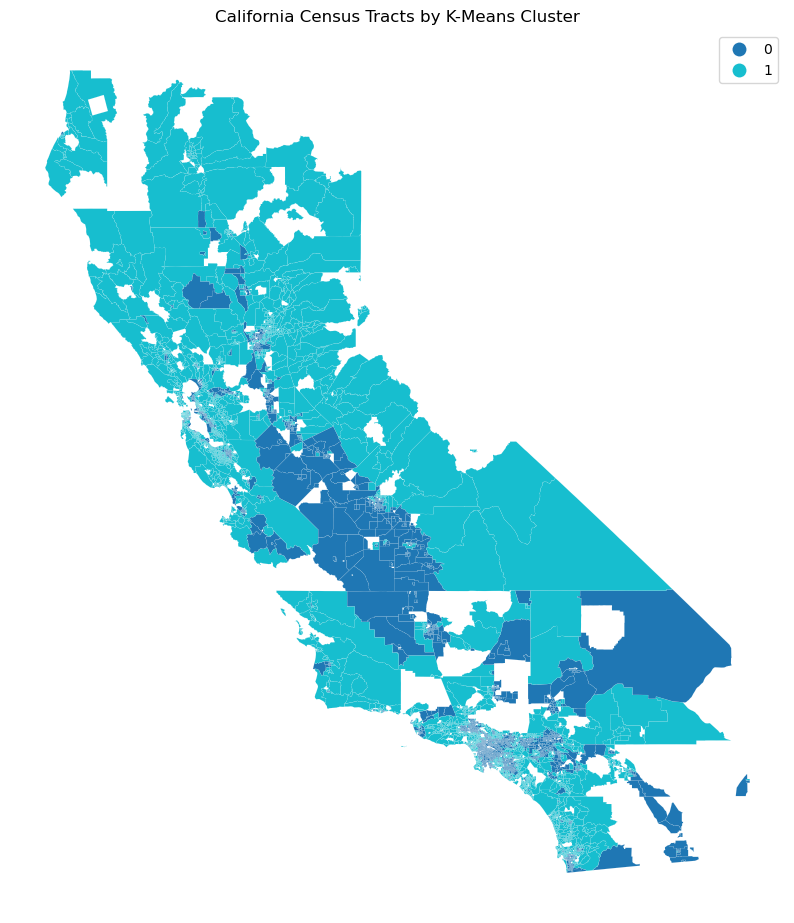
\includegraphics[width=0.7\linewidth]{files/1a4385a07d3ec64b034ce02d3597e6f8.png}

\begin{verbatim}
ax = gdf.plot(
    column="cluster_4",
    categorical=True,
    legend=True,
    figsize=(10, 12),
    linewidth=0.05,
    edgecolor="white"
)

ax.set_title("California Census Tracts by K -Means Cluster")
ax.set_axis_off()

plt.savefig("../visualizations/kmeans_visualizations/cluster_map_4.png", dpi=300, bbox_inches="tight")
plt.show()
\end{verbatim}

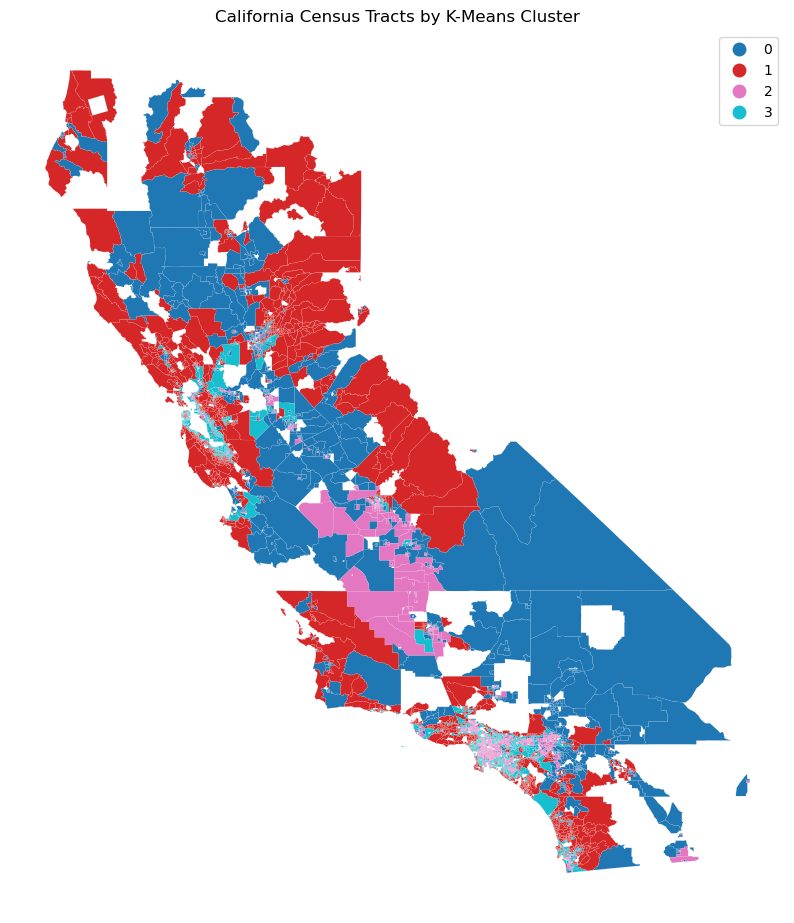
\includegraphics[width=0.7\linewidth]{files/eb0a8a2519718bdef75f4ae7fbaa0765.png}


\end{document}
